\documentclass[
	% -- opções da classe memoir --
	article,			% indica que é um artigo acadêmico
	11pt,				% tamanho da fonte
	oneside,			% para impressão apenas no recto. Oposto a twoside
	a4paper,			% tamanho do papel. 
	% -- opções da classe abntex2 --
	%chapter=TITLE,		% títulos de capítulos convertidos em letras maiúsculas
	%section=TITLE,		% títulos de seções convertidos em letras maiúsculas
	%subsection=TITLE,	% títulos de subseções convertidos em letras maiúsculas
	%subsubsection=TITLE % títulos de subsubseções convertidos em letras maiúsculas
	% -- opções do pacote babel --
	english,			% idioma adicional para hifenização
	brazil,				% o último idioma é o principal do documento
	sumario=tradicional
	]{abntex2}


% ---
% PACOTES
% ---

% ---
% Pacotes fundamentais 
% ---
\usepackage{lmodern}			% Usa a fonte Latin Modern
\usepackage[T1]{fontenc}		% Selecao de codigos de fonte.
\usepackage[utf8]{inputenc}		% Codificacao do documento (conversão automática dos acentos)
\usepackage{indentfirst}		% Indenta o primeiro parágrafo de cada seção.
\usepackage{nomencl} 			% Lista de simbolos
\usepackage{color}				% Controle das cores
\usepackage{graphicx}			% Inclusão de gráficos
\usepackage{microtype} 			% para melhorias de justificação
% ---
		
% ---
% Pacotes adicionais, usados apenas no âmbito do Modelo Canônico do abnteX2
% ---
\usepackage{lipsum}				% para geração de dummy text
% ---
		
% ---
% Pacotes de citações
% ---
\usepackage[brazilian,hyperpageref]{backref}	 % Paginas com as citações na bibl
\usepackage[alf]{abntex2cite}	% Citações padrão ABNT
% ---

% ---
% Configurações do pacote backref
% Usado sem a opção hyperpageref de backref
\renewcommand{\backrefpagesname}{Citado na(s) página(s):~}
% Texto padrão antes do número das páginas
\renewcommand{\backref}{}
% Define os textos da citação
\renewcommand*{\backrefalt}[4]{
	\ifcase #1 %
		Nenhuma citação no texto.%
	\or
		Citado na página #2.%
	\else
		Citado #1 vezes nas páginas #2.%
	\fi}%
% ---

% --- Informações de dados para CAPA e FOLHA DE ROSTO ---
\title{Modelo Matemático de um Cooktop Indutivo}

\author{Myke Albuquerque Pinto de Oliveira}

\local{Brasil}
\data{2019, 0.0}
% ---

% ---
% Configurações de aparência do PDF final

% alterando o aspecto da cor azul
\definecolor{blue}{RGB}{41,5,195}

% informações do PDF
\makeatletter
\hypersetup{
     	%pagebackref=true,
		pdftitle={\@title}, 
		pdfauthor={\@author},
    	pdfsubject={Modelo Matemático de um Cooktop Indutivo},
	    pdfcreator={LaTeX with abnTeX2},
		pdfkeywords={cooktop}{indução}{eletromagnetismo}{modelagem matemática}{física}, 
		colorlinks=true,       		% false: boxed links; true: colored links
    	linkcolor=blue,          	% color of internal links
    	citecolor=blue,        		% color of links to bibliography
    	filecolor=magenta,      		% color of file links
		urlcolor=blue,
		bookmarksdepth=4
}
\makeatother
% --- 

% ---
% compila o indice
% ---
\makeindex
% ---

% ---
% Altera as margens padrões
% ---
\setlrmarginsandblock{3cm}{3cm}{*}
\setulmarginsandblock{3cm}{3cm}{*}
\checkandfixthelayout
% ---

% --- 
% Espaçamentos entre linhas e parágrafos 
% --- 

% O tamanho do parágrafo é dado por:
\setlength{\parindent}{1.3cm}

% Controle do espaçamento entre um parágrafo e outro:
\setlength{\parskip}{0.2cm}  % tente também \onelineskip

% Espaçamento simples
\SingleSpacing


% ----
% Início do documento
% ----
\begin{document}

% Seleciona o idioma do documento (conforme pacotes do babel)
%\selectlanguage{english}
\selectlanguage{brazil}

% Retira espaço extra obsoleto entre as frases.
\frenchspacing 

% ----------------------------------------------------------
% ELEMENTOS PRÉ-TEXTUAIS
% ----------------------------------------------------------

%---
%
% Se desejar escrever o artigo em duas colunas, descomente a linha abaixo
% e a linha com o texto ``FIM DE ARTIGO EM DUAS COLUNAS''.
% \twocolumn[    		% INICIO DE ARTIGO EM DUAS COLUNAS
%
%---

% página de titulo principal (obrigatório)
\maketitle


% titulo em outro idioma (opcional)



% resumo em português
\begin{resumoumacoluna}
 Conforme a ABNT NBR 6022:2018, o resumo no idioma do documento é elemento obrigatório. 
 Constituído de uma sequência de frases concisas e objetivas e não de uma 
 simples enumeração de tópicos, não ultrapassando 250 palavras, seguido, logo 
 abaixo, das palavras representativas do conteúdo do trabalho, isto é, 
 palavras-chave e/ou descritores, conforme a NBR 6028. (\ldots) As 
 palavras-chave devem figurar logo abaixo do resumo, antecedidas da expressão 
 Palavras-chave:, separadas entre si por ponto e finalizadas também por ponto.
 
 \vspace{\onelineskip}
 
 \noindent
 \textbf{Palavras-chave}: cooktop, indução, eletromagnetismo, modelagem matemática, física.
\end{resumoumacoluna}


% resumo em inglês
\renewcommand{\resumoname}{Abstract}
\begin{resumoumacoluna}
 \begin{otherlanguage*}{english}
   According to ABNT NBR 6022:2018, an abstract in foreign language is optional.

   \vspace{\onelineskip}
 
   \noindent
   \textbf{Keywords}: cook-top, induction, electromagnetism, mathematical model, physics.
 \end{otherlanguage*}  
\end{resumoumacoluna}

% ]  				% FIM DE ARTIGO EM DUAS COLUNAS
% ---

\begin{center}\smaller
\textbf{Data de submissão e aprovação}: elemento obrigatório. Indicar dia, mês e ano

\textbf{Identificação e disponibilidade}: elemento opcional. Pode ser indicado 
o endereço eletrônico, DOI, suportes e outras informações relativas ao acesso.
\end{center}

% ----------------------------------------------------------
% ELEMENTOS TEXTUAIS
% ----------------------------------------------------------
\textual

% ----------------------------------------------------------
% Introdução
% ----------------------------------------------------------
\section{Introdução}

Um cooktop de indução (informalmente fogão de indução) é um equipamento que substitui o fogão no preparo de alimentos. O cooktop de indução difere do cooktop a gás porque sua fonte de energia é a eletricidade e não o gás liquefeito de petróleo, e também difere do cooktop elétrico por resistência, pois ao invés de possuir uma superfície metálica aquecida por uma resistência elétrica, o cooktop de indução não apresenta nenhuma superfície aquecida além da própria panela onde o alimento está sendo preparado. O princípio de funcionamento do cooktop de indução é baseado na geração de um campo magnético variável através de uma bobina espiralada e a geração de um campo elétrico induzido no material da panela, esse campo elétrico, por sua vez, gera correntes elétricas na panela e calor por efeito Joule.

Entre as vantangens de se adotar um cooktop de indução, pode-se citar:

\begin{itemize}
	\item Dispensa o uso de botijão de gás.
	\item Não há superfícies quentes no equipamento e não funciona sem a presença da panela no equipamento.
	\item Melhor eficiência no aquecimento, pois não perde calor na transferência por convecção.
	\item A maioria dos modelos é microcontrolada e fornece opções como o desligamento temporizado e o controle automático de potência.
\end{itemize}

O presente artigo é o resultado de discussão e pesquisa da Unidade de Aprendizagem "Resolução de Problemas no Contexto da Física" e tem como objetivo estabelecer a relação entre a corrente elétrica que circula na bobina espiralada do cooktop de indução e a potência calórica fornecida. Incluindo essa introdução, o artigo está dividido em cinco seções, a segunda seção apresenta mais detalhes sobre o problema a ser resolvido. A terceira seção resolve detalhadamente o problema. A quarta seção fecha este artigo sob a ótica educativa e de formação de competências.

\section{Problema de estudo}

\subsection{Enunciado do problema}

Dado um condutor elétrico $ L $ de formato espiralado percorrido por uma corrente $ i(t) $ e uma chapa $ C $ sobre esse condutor, conforme figura \ref{fig:fig1}. Estabelecer a relação entre a corrente $ i(t) $ e a potência de calor $ P(t) $ gerada na chapa metálica.

\begin{figure}[h]
	\centering
	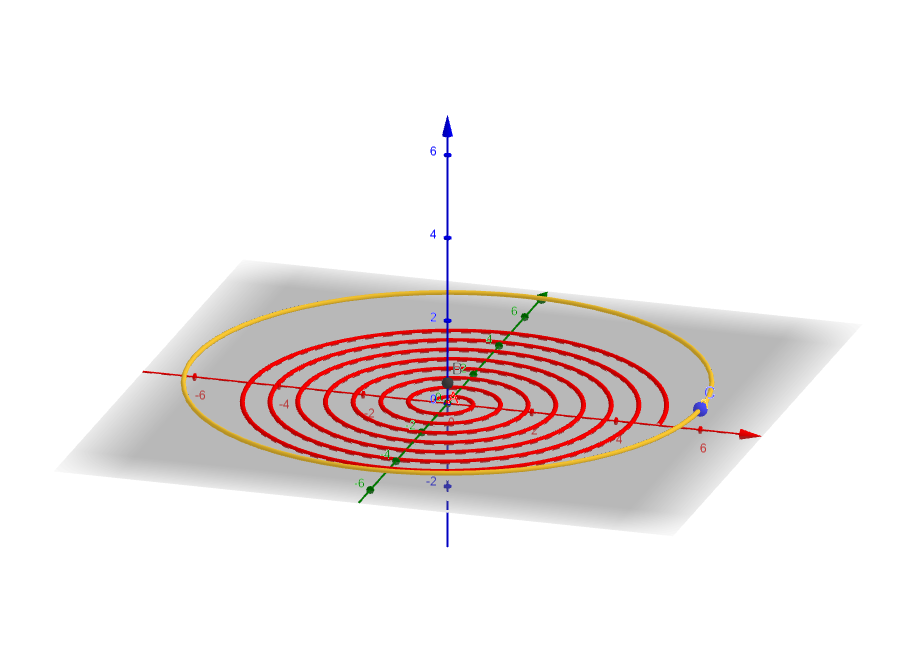
\includegraphics[width=0.7\linewidth]{figures/fig1}
	\caption[Esquema de um cooktop de indução]{Esquema de um cooktop de indução}
	\label{fig:fig1}
\end{figure}

\subsection{Tema que contextualiza o problema}

\subsection{Objetos de Estudos}

\subsection{Variáveis e parâmetros do problema}

\textbf{Parâmetros que definem o problema:}

\begin{itemize}
	\item[$ N $] número de espiras na bobina
	\item[$ e $] espaçamento radial entre as bobinas
	\item[$ d $] distância entre a bobina e o fundo da panela.
\end{itemize}

\textbf{Variáveis associadas ao problema:}

\begin{itemize}
	\item[$ t $] tempo, variável independente.
	\item[$ i(t) $] corrente elétrica que circula o condutor espiradado.
	\item[$ \vec{B}(t) $] campo magnético gerado.
	\item[$ \vec{E}(t) $] campo elétrico.
	\item[$ \vec{J}(t) $] densidade de corrente elétrica
	\item[$ P(t) $] potência calorifica gerada na panela
\end{itemize}

\section{Resolução detalhada do problema}

\section{Análise e considerações finais}

\section{REFERÊNCIAS BIBLIOGRÁFICAS}

\end{document}
